\documentclass[ignorenonframetext,]{beamer}
\setbeamertemplate{caption}[numbered]
\setbeamertemplate{caption label separator}{: }
\setbeamercolor{caption name}{fg=normal text.fg}
\beamertemplatenavigationsymbolsempty
\usepackage{lmodern}
\usepackage{amssymb,amsmath}
\usepackage{ifxetex,ifluatex}
\usepackage{fixltx2e} % provides \textsubscript
\ifnum 0\ifxetex 1\fi\ifluatex 1\fi=0 % if pdftex
\usepackage[T1]{fontenc}
\usepackage[utf8]{inputenc}
\else % if luatex or xelatex
\ifxetex
\usepackage{mathspec}
\else
\usepackage{fontspec}
\fi
\defaultfontfeatures{Ligatures=TeX,Scale=MatchLowercase}
\fi
\usetheme{Madrid}
\usecolortheme{seahorse}
\usefonttheme{serif}
% use upquote if available, for straight quotes in verbatim environments
\IfFileExists{upquote.sty}{\usepackage{upquote}}{}
% use microtype if available
\IfFileExists{microtype.sty}{%
\usepackage{microtype}
\UseMicrotypeSet[protrusion]{basicmath} % disable protrusion for tt fonts
}{}
\newif\ifbibliography
\usepackage{natbib}
\bibliographystyle{plainnat}

% Prevent slide breaks in the middle of a paragraph:
\widowpenalties 1 10000
\raggedbottom

\AtBeginPart{
\let\insertpartnumber\relax
\let\partname\relax
\frame{\partpage}
}
\AtBeginSection{
\ifbibliography
\else
\let\insertsectionnumber\relax
\let\sectionname\relax
\frame{\sectionpage}
\fi
}
\AtBeginSubsection{
\let\insertsubsectionnumber\relax
\let\subsectionname\relax
\frame{\subsectionpage}
}

\setlength{\parindent}{0pt}
\setlength{\parskip}{6pt plus 2pt minus 1pt}
\setlength{\emergencystretch}{3em}  % prevent overfull lines
\providecommand{\tightlist}{%
\setlength{\itemsep}{0pt}\setlength{\parskip}{0pt}}
\setcounter{secnumdepth}{0}
\usepackage{textpos}
\usepackage{mathpazo}

\definecolor{first}{HTML}{009D7F}
\definecolor{first-text}{HTML}{F2F2F2}
\definecolor{second}{HTML}{00997D}
\definecolor{second-text}{HTML}{FDFDFD}
\definecolor{third}{HTML}{008068}
\definecolor{third-text}{HTML}{FFFFFF}
\setbeamercolor*{palette primary}{use=structure,fg=first-text,bg=first}
\setbeamercolor*{palette secondary}{use=structure,fg=second-text,bg=second}
\setbeamercolor*{palette tertiary}{use=structure,fg=third-text,bg=third}
\setbeamercolor{item projected}{fg=white,bg=third}

\addtobeamertemplate{frametitle}{}{%
\begin{textblock*}{100mm}(0.92\textwidth,-0.85cm)

\includegraphics[height=0.75cm]{images/LogoNMBUwhite}
\end{textblock*}}

\titlegraphic{
\includegraphics[height=1cm]{images/LogoNMBU}}
% \renewcommand*{\bibfont}{\scriptsize}

\makeatletter
\setbeamertemplate{footline}
{
  \leavevmode%
  \hbox{%
  \begin{beamercolorbox}[wd=.15\paperwidth,ht=2.25ex,dp=1ex,center]{author in head/foot}%
    \usebeamerfont{author in head/foot}\insertshortauthor
  \end{beamercolorbox}%
  \begin{beamercolorbox}[wd=.6\paperwidth,ht=2.25ex,dp=1ex,center]{title in head/foot}%
    \usebeamerfont{title in head/foot}\inserttitle
  \end{beamercolorbox}%
  \begin{beamercolorbox}[wd=.25\paperwidth,ht=2.25ex,dp=1ex,right]{date in head/foot}%
    \usebeamerfont{date in head/foot}\insertshortdate{}\hspace*{2em}
    \insertframenumber{} / \inserttotalframenumber\hspace*{2ex} 
  \end{beamercolorbox}}%
  \vskip0pt%
}
\makeatother

\title{PhD Midway Seminar}
\subtitle{Simulation Tool and its application}
\author{Raju Rimal}
\institute{\textbf{Supervisors}\\
Solve Sæbø, Tryge Almøy}
\date{04 March, 2017}

\begin{document}
\frame{\titlepage}

\section{Introduction}\label{introduction}

\begin{frame}{My PhD Plan}

\hypertarget{left}{}

\hypertarget{right}{}
\begin{itemize}[<+->]
\tightlist
\item
  Make {Simulation Tools} for multi-response linear model data
\item
  Using the tool, compare various {estimation techniques} and
  {understand} them
\item
  {Extend} the simulation tool incorporating model with {background
  information}
\item
  Apply this extended tool to {test multi-matrix extension of partial
  least square (PLS)} models such as LPLS and UPLS (both uses background
  information about \(X\) and \(Y\) for analysis)
\end{itemize}

\begin{block}{Comment on PLS in short}

\end{block}

\end{frame}

\begin{frame}{What I learn}

\begin{itemize}[<+->]
\tightlist
\item
  Advanced Multivariate Model and technique to analyze it
\item
  Programming concept for developing statistical packages and
  applications for various statistical methods
\item
  Extending and improving existing methods in statistics
\item
  And, obviously, to properly document what I have done
\end{itemize}

\end{frame}

\begin{frame}[fragile]{Today's Special}

Today I will talk about:

\begin{itemize}[<+->]
\tightlist
\item
  Simulation tool ({\texttt{simulatr}}) we are building
\item
  A {comparative study} of various estimation techniques by simulating
  linear model data using \texttt{simulatr}
\end{itemize}

\end{frame}

\section{\texorpdfstring{\texttt{simrel-m}: A versatile tool for
simulating multi-response linear model
data}{simrel-m: A versatile tool for simulating multi-response linear model data}}\label{simrel-m-a-versatile-tool-for-simulating-multi-response-linear-model-data}

\begin{frame}[fragile]{Overview}

\pause

\texttt{simrel-M} is an extension of \texttt{simrel}
\citep{saebo2015simrel} r-package for simulating multi-response data

\begin{itemize}
\tightlist
\item
  Uses the idea of reduction of random regression model by separating
  latent space of \(\mathbf{X}\) into subspaces that is relevant and
  irrelevant for predicting each response
\item
  The underlying concept is based on reparameterizing the population
  model,
\end{itemize}

\[
\mathbf{Y} = \boldsymbol{\mu}_{Y} + \mathbf{B}^t\left(\mathbf{X} - \boldsymbol{\mu}_X\right) + \boldsymbol{\epsilon}
\text{, where }\boldsymbol{\epsilon} \sim N(0, \boldsymbol{\Sigma}_{Y|X})
\]

\end{frame}

\begin{frame}{Underlying procedure}

\pause

\hypertarget{left}{}

\hypertarget{right}{}
\begin{itemize}[<+->]
\tightlist
\item
  Collect population input parameter from users such as: number of
  variables, coefficient of determination and the position of relevant
  components
\item
  Make a covariance matrix satisfying input parameters
\item
  Rotate the covariance matrix orthogonally
\item
  Sample calibration and validation sets
\end{itemize}

\end{frame}

\section{A comparative study of different estimation methods using
simulated
data}\label{a-comparative-study-of-different-estimation-methods-using-simulated-data}

\begin{frame}{Overview}

\begin{block}{Four estimtion methods were considered}

\hypertarget{left}{}
\paragraph{Ordinary Least Squares
(OLS)}\label{ordinary-least-squares-ols}

\begin{itemize}
\tightlist
\item
  Although unbiased, suffer highly from multicollinearity
\item
  Widely used and can be used as reference for comparison
\end{itemize}

\paragraph{Envelope}\label{envelope}

\begin{itemize}
\tightlist
\item
  Relatively new method \citep{cook2013envelopes} and is also based on
  reduction of regression model
\item
  Based on Maximum Likelihood but works better than OLS in \(p\)
  approaches \(n\)
\end{itemize}

\hypertarget{right}{}
\paragraph{Partial Least Squares (PLS)}\label{partial-least-squares-pls}

\begin{itemize}
\tightlist
\item
  Well established and widely used method
\item
  Based on Latent Structure and free of multicollinearity problem
\end{itemize}

\paragraph{Bayes PLS}\label{bayes-pls}

\begin{itemize}
\tightlist
\item
  Bayesian Estimation of regression coefficient
\item
  Promising performance was shown in previous studies
  \citep{helland2012near}
\end{itemize}

\end{block}

\end{frame}

\begin{frame}{Simulation Design}

\pause

From the possible combination of following parameter combination,
\emph{32} single response calibration sets were simulated with \emph{5}
replication of each.

\begin{itemize}[<+->]
\tightlist
\item
  \textbf{Number of sample observations}: \emph{50}
\item
  \textbf{Number of predictor variables}: \emph{15} and \emph{40}
\item
  \textbf{Coefficient of determination \((R^2)\)}: \emph{0.5} and
  \emph{0.9}
\item
  \textbf{Level of multicollinearity}: \emph{0.5} and \emph{0.9}
\item
  \textbf{Position of relevant components}: \emph{1} and \emph{2};
  \emph{1} and \emph{3}; \emph{2} and \emph{3}; \emph{1}, \emph{2} and
  \emph{3}
\end{itemize}

\begin{block}{Coefficient of determination denotes information level in
the simulated dataset}

\end{block}

\begin{block}{Lower the value of level of multicollinearity, better
(i.e.~predictor variables are independent) and also supports assumption
of linear model}

\end{block}

\end{frame}

\begin{frame}{A Systematic Comparison}

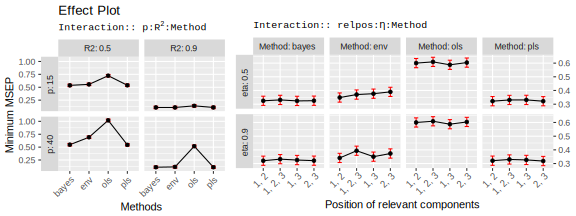
\includegraphics[width=0.6\linewidth]{images/effect-plot}

\hypertarget{left}{}
\begin{itemize}
\tightlist
\item
  Bayes PLS has out-performed others methods in all kinds of data
\item
  Envelope has performed better than OLS in all situations and PLS in
  some situations
\end{itemize}

\hypertarget{right}{}
\begin{itemize}
\tightlist
\item
  OLS prediction is very poor in noisy data with many predictor
  variables
\item
  Position of relvant component and the decaying factor of eigenvalue
  has less impact on prediction in all the models
\end{itemize}

\begin{block}{Small prediction error gives good result and is better}

\end{block}

\end{frame}

\begin{frame}{A Systematic Comparison}

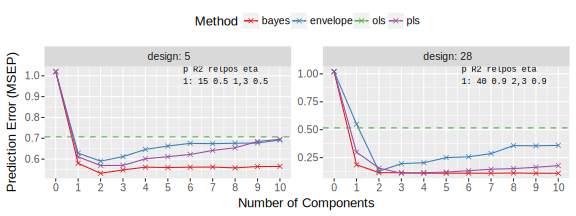
\includegraphics[width=0.6\linewidth]{images/prediction-error-selected}

\hypertarget{left}{}
\begin{itemize}
\tightlist
\item
  Bayes PLS has approached to its minimum error with very few component
  and remained low for additional component
\item
  PLS has moderate performance but better than envelope in many
  situations.
\end{itemize}

\hypertarget{right}{}
\begin{itemize}
\tightlist
\item
  OLS prediction is poor especially with large number of predictor
\item
  Envelope method captured its minimum error and the error increased
  with additional components
\end{itemize}

\begin{block}{Number of components are the assumed dimension of relevant
x-space}

\end{block}

\end{frame}

\section{Demonstration}\label{demonstration}

\begin{frame}{\texttt{simulatr} Application}

\end{frame}

\section{}\label{section}

\section{References}\label{references}

\begin{frame}{References}

\end{frame}

\begin{frame}[allowframebreaks]{}
\bibliographytrue
\bibliography{references.bib}
\end{frame}

\end{document}
